\chapter{Architectural Design}

\section{Overview}
The system will be developed from scratch and it will completely replace the legacy system. \newline

\vspace{0.8em}
\begin{figure}[H]
	\centering
	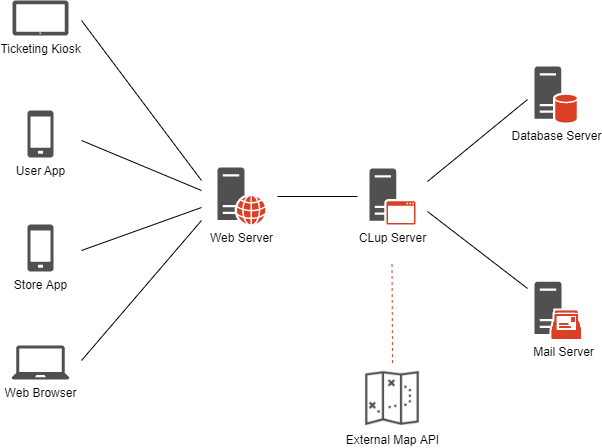
\includegraphics[scale=0.45]{overview_diagram}
	\caption{CLup system diagram.}
\end{figure}


It is composed by a client part and a server part:
\begin{itemize}
	\item \textbf{Server side:}
	\begin{itemize}
		\item \textit{Application Server (CLup Server):} server where all the logic is located. It communicates with other servers and is the central point of the system.
		\item \textit{Web Server:} server used for the communication with the clients.
		\item \textit{Database Server:} server where all data are stored.
		\item \textit{Mail Server:} server used to send confirmation emails about the bookings.
		\item \textit{External map API:} API used to retrieve data about the distance of the user from the store. This information will be used to inform the user of when leave the current place.
	\end{itemize}
	\item \textbf{Client side:}
	\begin{itemize}
		\item \textit{User App:} Application installed on customers smartphone. It allows to retrieve a ticket or book a visit.
		\item \textit{Store App:} Application installed on employees smartphone. It allows to validate store passes.
		\item \textit{Ticketing Kiosk:} Tablet installed at the entrance of the store to which a printer is attached. It has installed a modified version of the mobile app which is able to print the ticket on place.
		\item \textit{Web Browser:} Used by store employees and managers to access the web dashboard.
	\end{itemize}
\end{itemize}

\section{Component view}

\section{Deployment view}

\clearpage
\section{Runtime view}
This section describes the most important components interactions of the system.\newline
For the sake of simplicity the sequence diagrams are based on the first level of components. 
\subsection{Customer App token}
At the startup, the Customer App will try to request a token to the server via the token manager. Having a token is mandatory in order to take any action with the app.\newline
This process is really important because the token is the only way to identify a customer since no registration is expected. The app will reiterate the process till a valid token is gotten.\newline
This is an automatic process and no action is performed by the user during the operation.
\begin{figure}[H]
	\centering
	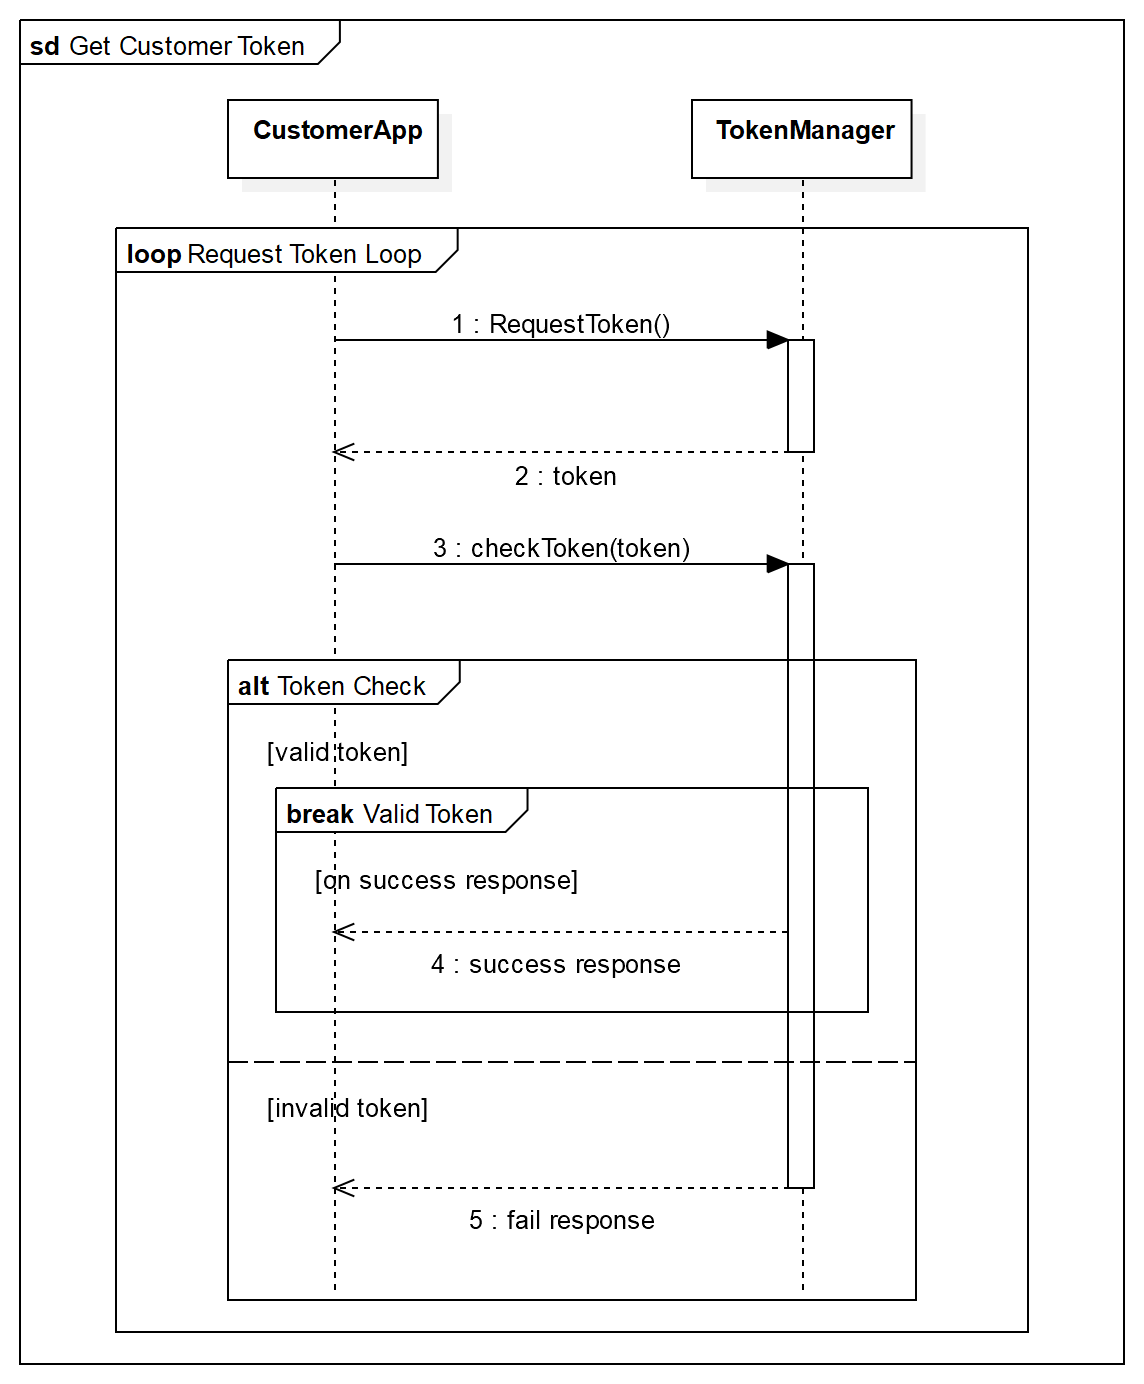
\includegraphics[width=0.8\linewidth]{token_seq}
	\caption{Customer app token request.}
	\label{fig:token_seq}
\end{figure}
\clearpage

\subsection{Ticket request}
The request for a ticket starts from the Customer App and contains both token and selected store. The token validation is the first operation performed by the server and consequently, if all the checks go well, a ticket is retrieved.
\vspace{0.1cm}
\begin{figure}[H]
	\centering
	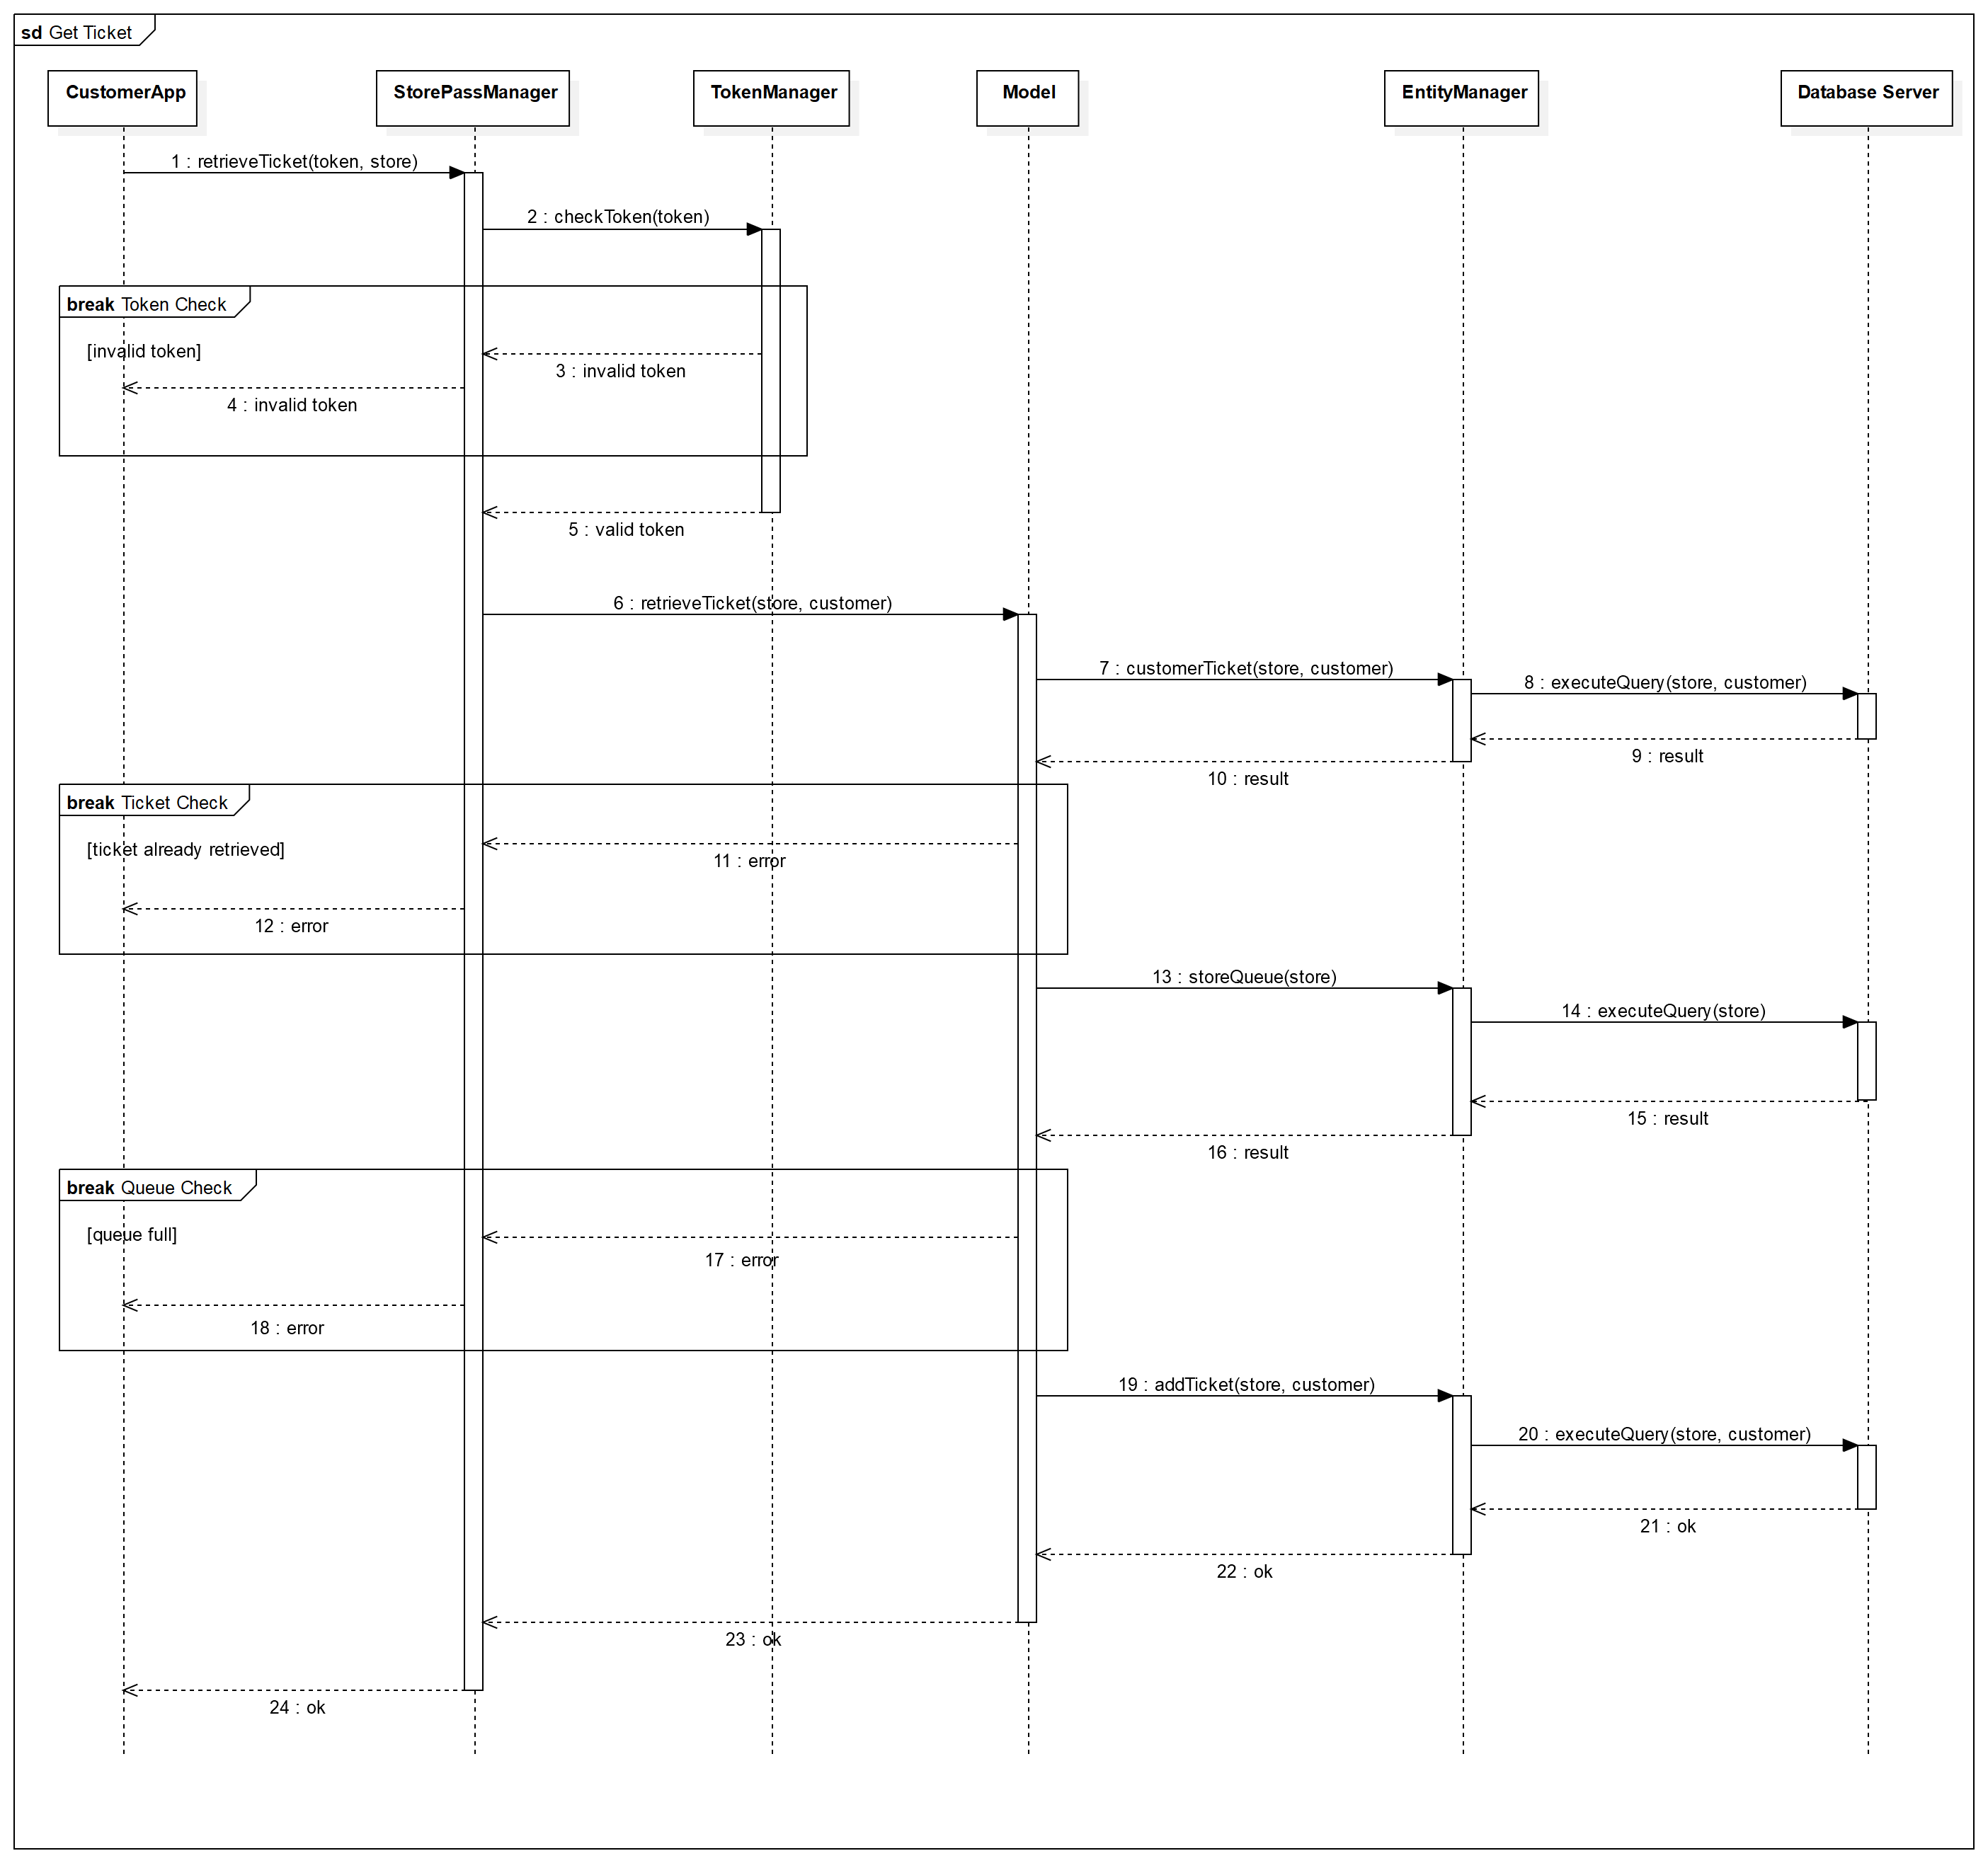
\includegraphics[width=\linewidth]{ticket_seq}
	\caption{Ticket request.}
	\label{fig:ticket_seq}
\end{figure}

\clearpage

\subsection{Booking request}
A user can book a visit for a store if he hasn't booked a visit to the same store and in the same day yet. This check is done together with the token validation and others checks.\newline
Since a booking must be confirmed via a link, an email is sent at the end of the whole process through the mail server.
\begin{figure}[H]
	\centering
	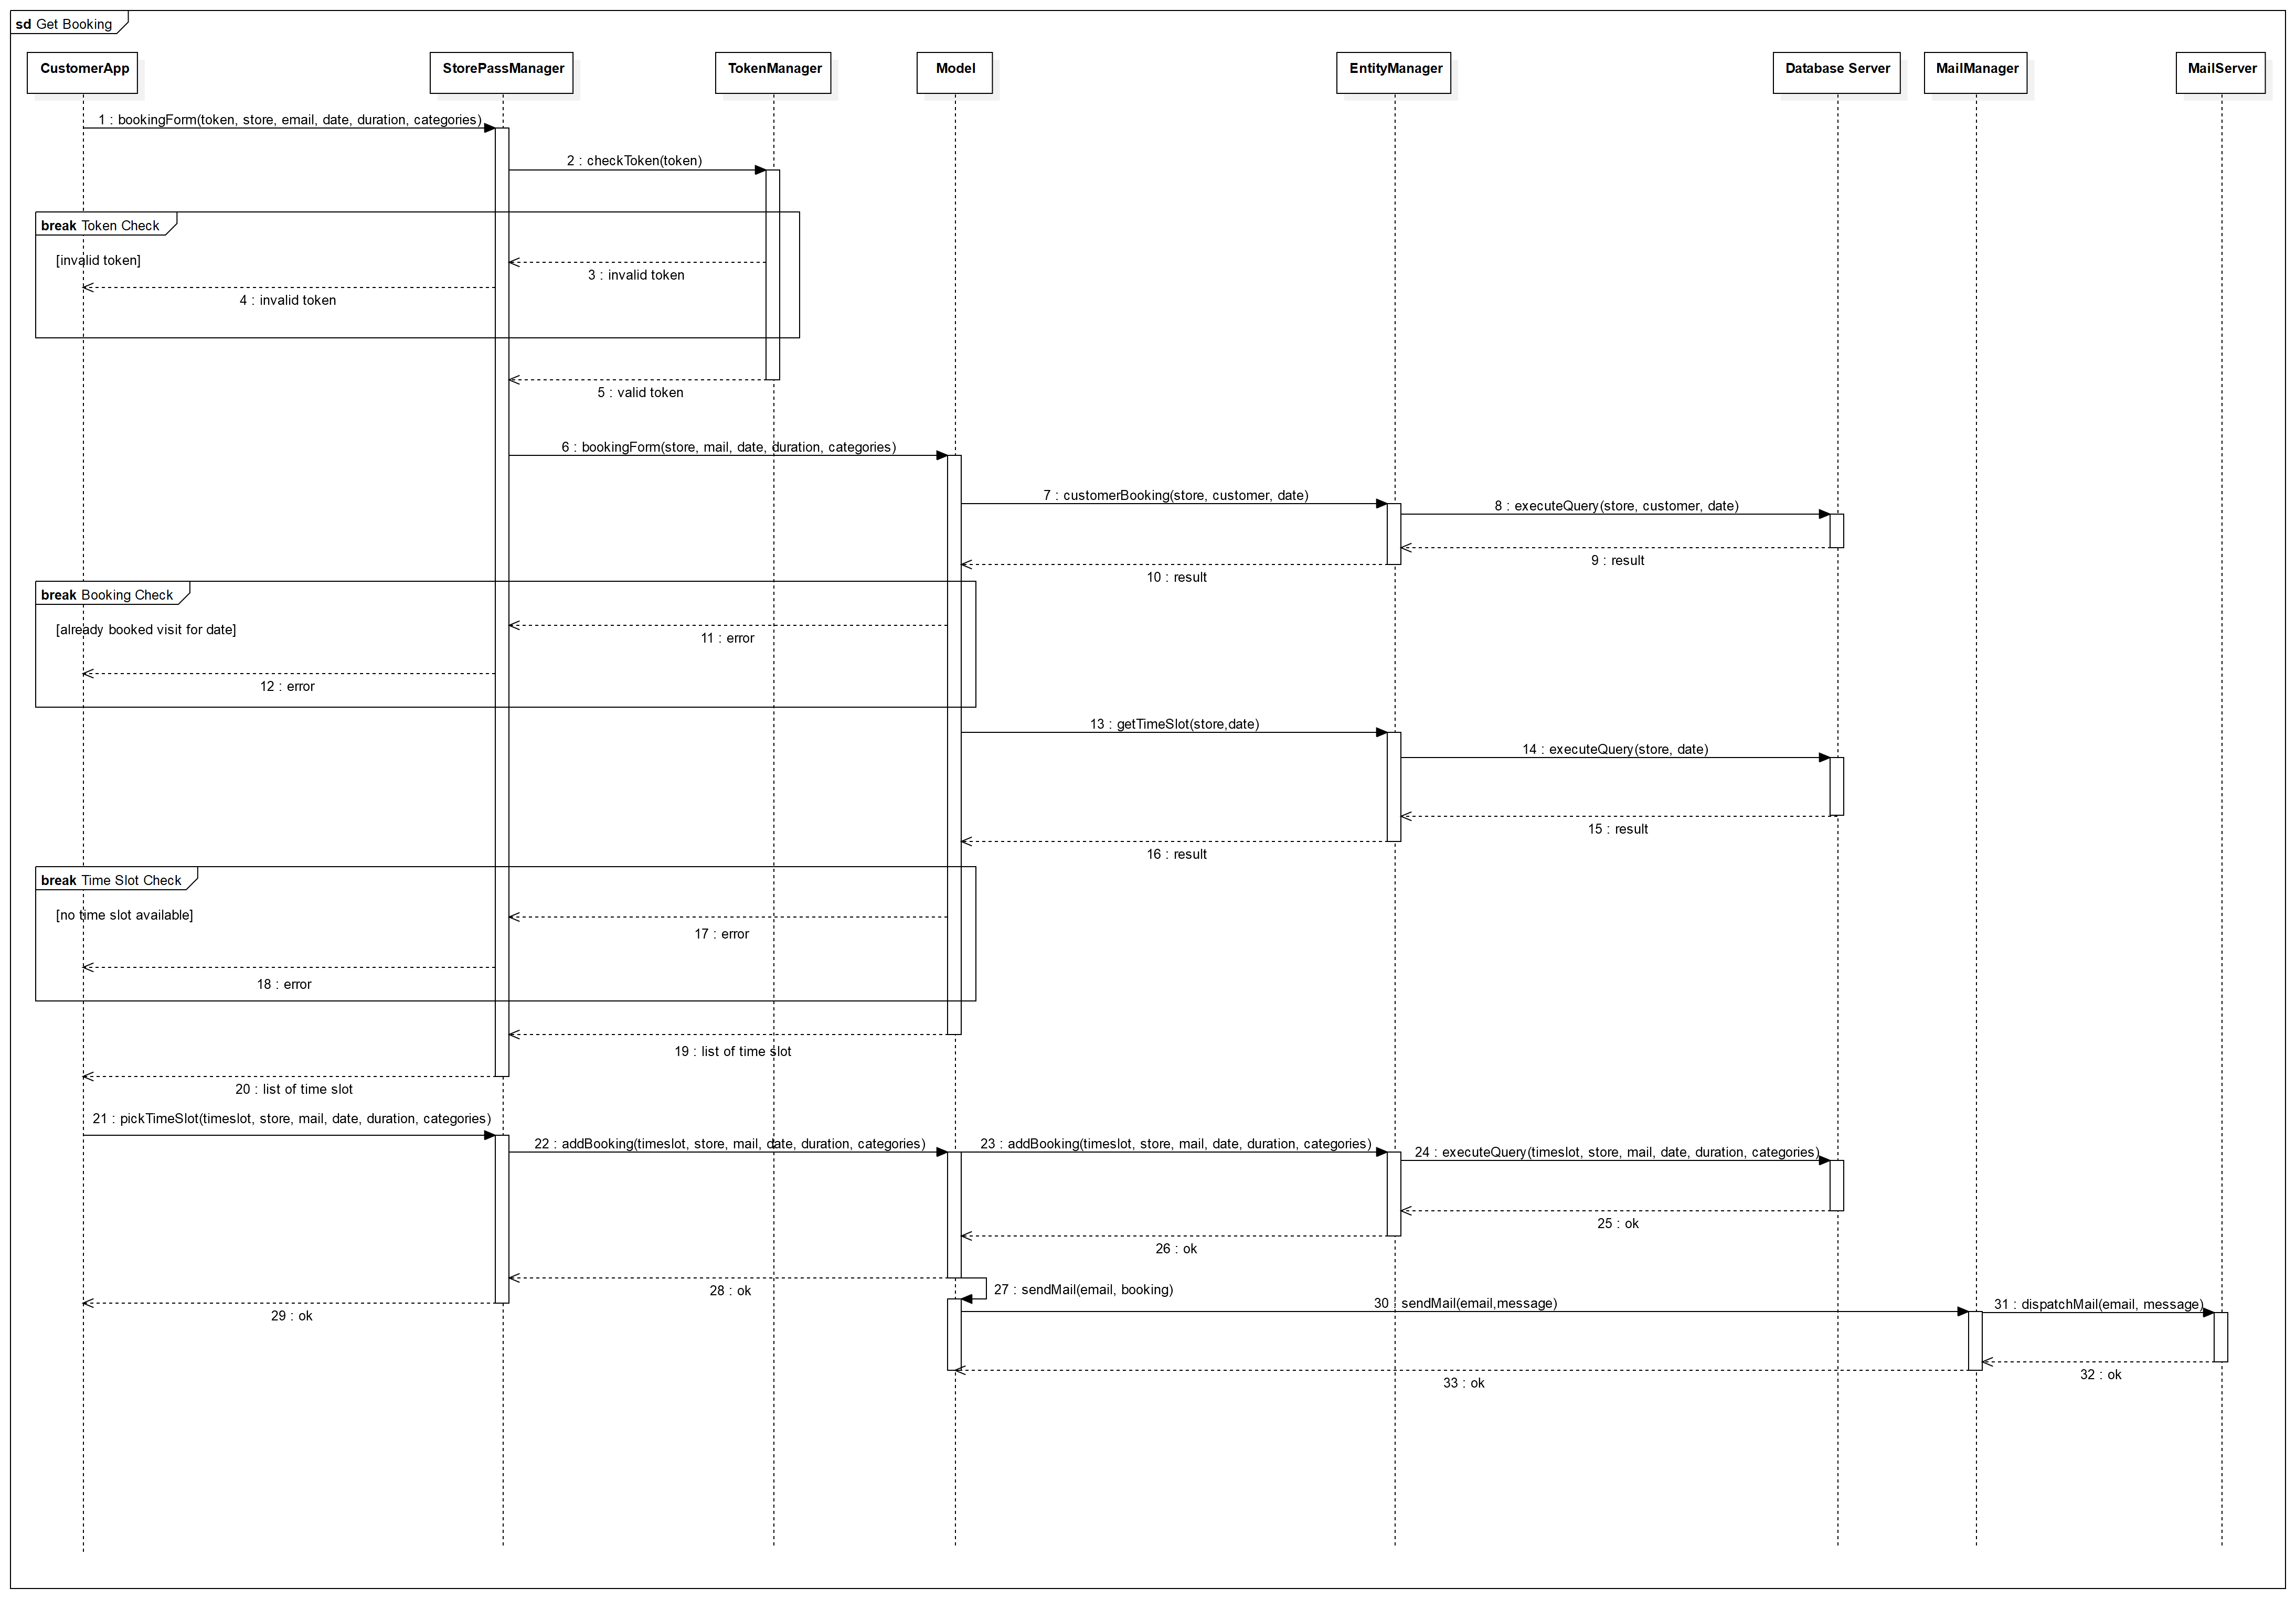
\includegraphics[angle=90,origin=c,height=\linewidth]{booking_seq}
	\caption{Booking request.}
	\label{fig:booking_seq}
\end{figure}

\clearpage
\subsection{Leave At Time}
The Customer App reminds the user to leave the place where he is in order to ensure that he arrives on time.\newline
The server fetches all the valid store passes and computes the distance of the customer from the respective store. If the customer should leave the place where he is, a notification is sent to him.
\begin{figure}[H]
	\centering
	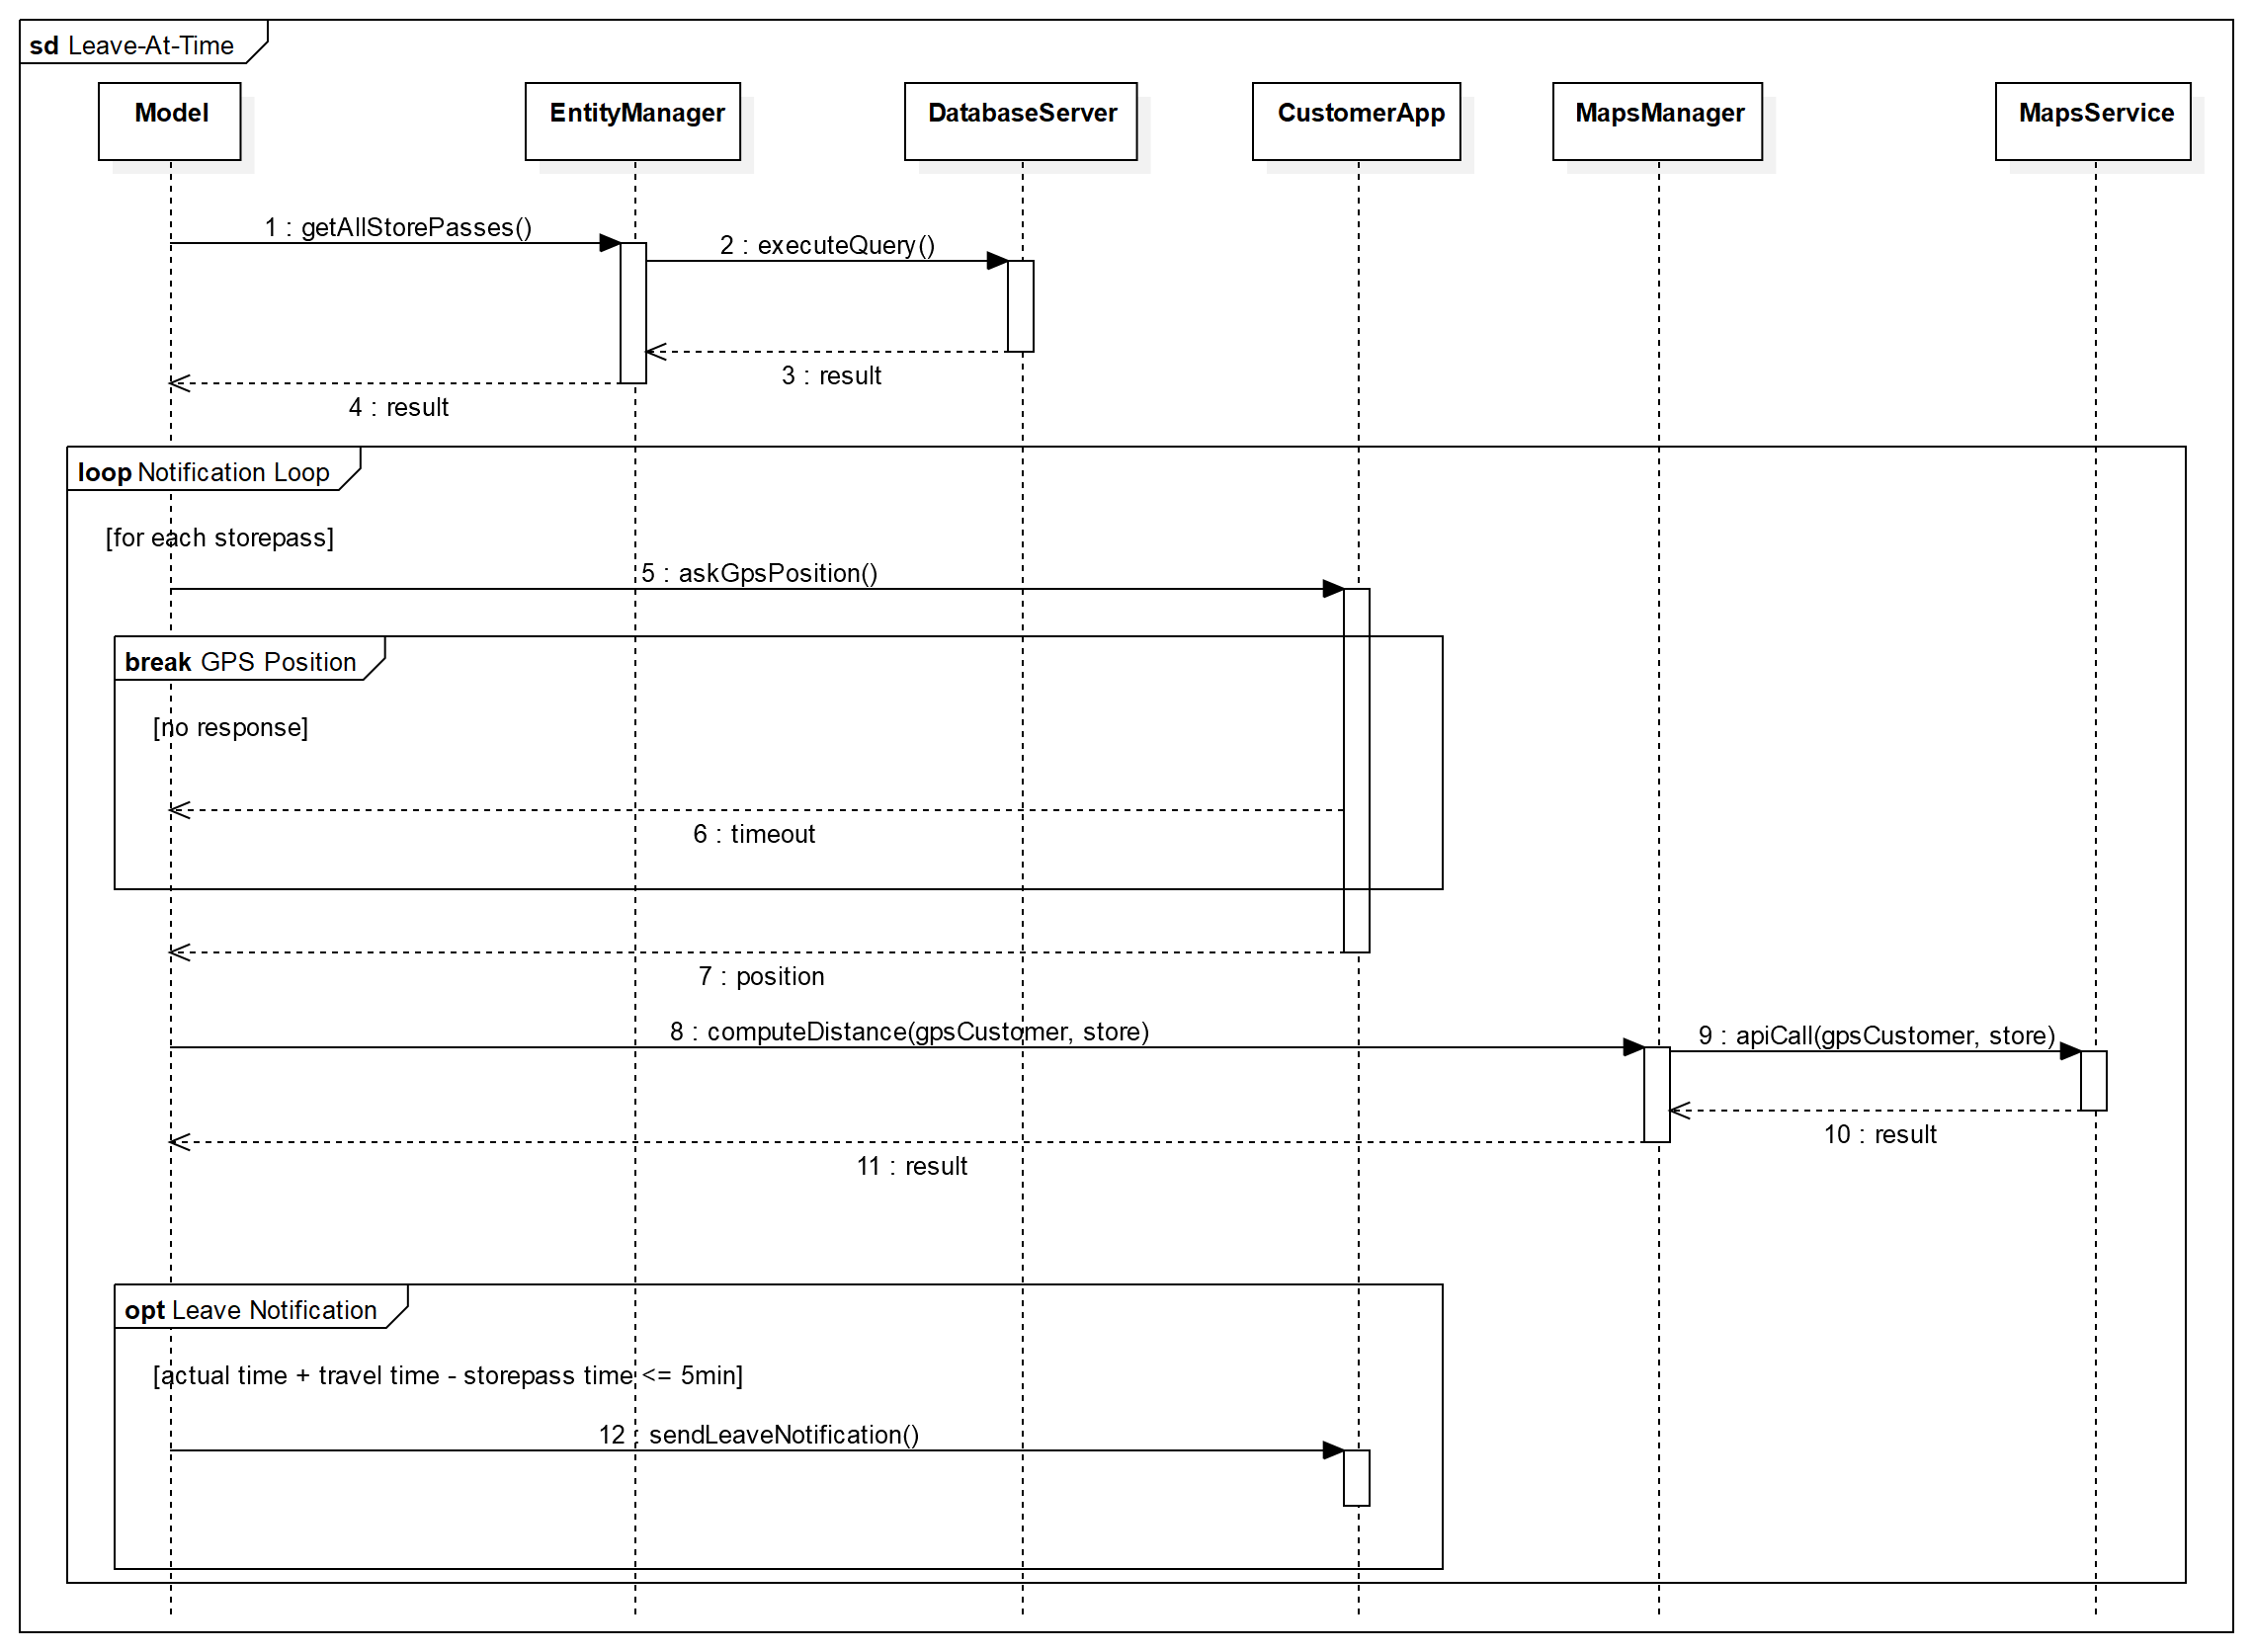
\includegraphics[width=0.75\linewidth]{leave_seq}
	\caption{Leave at time function.}
	\label{fig:leave_seq}
\end{figure}

\subsection{Web App login}
The following sequence diagram represents the login process to the Web App. CLup admins, store managers and store employees will authenticate to the system by submitting their credentials via a form.
\begin{figure}[H]
	\centering
	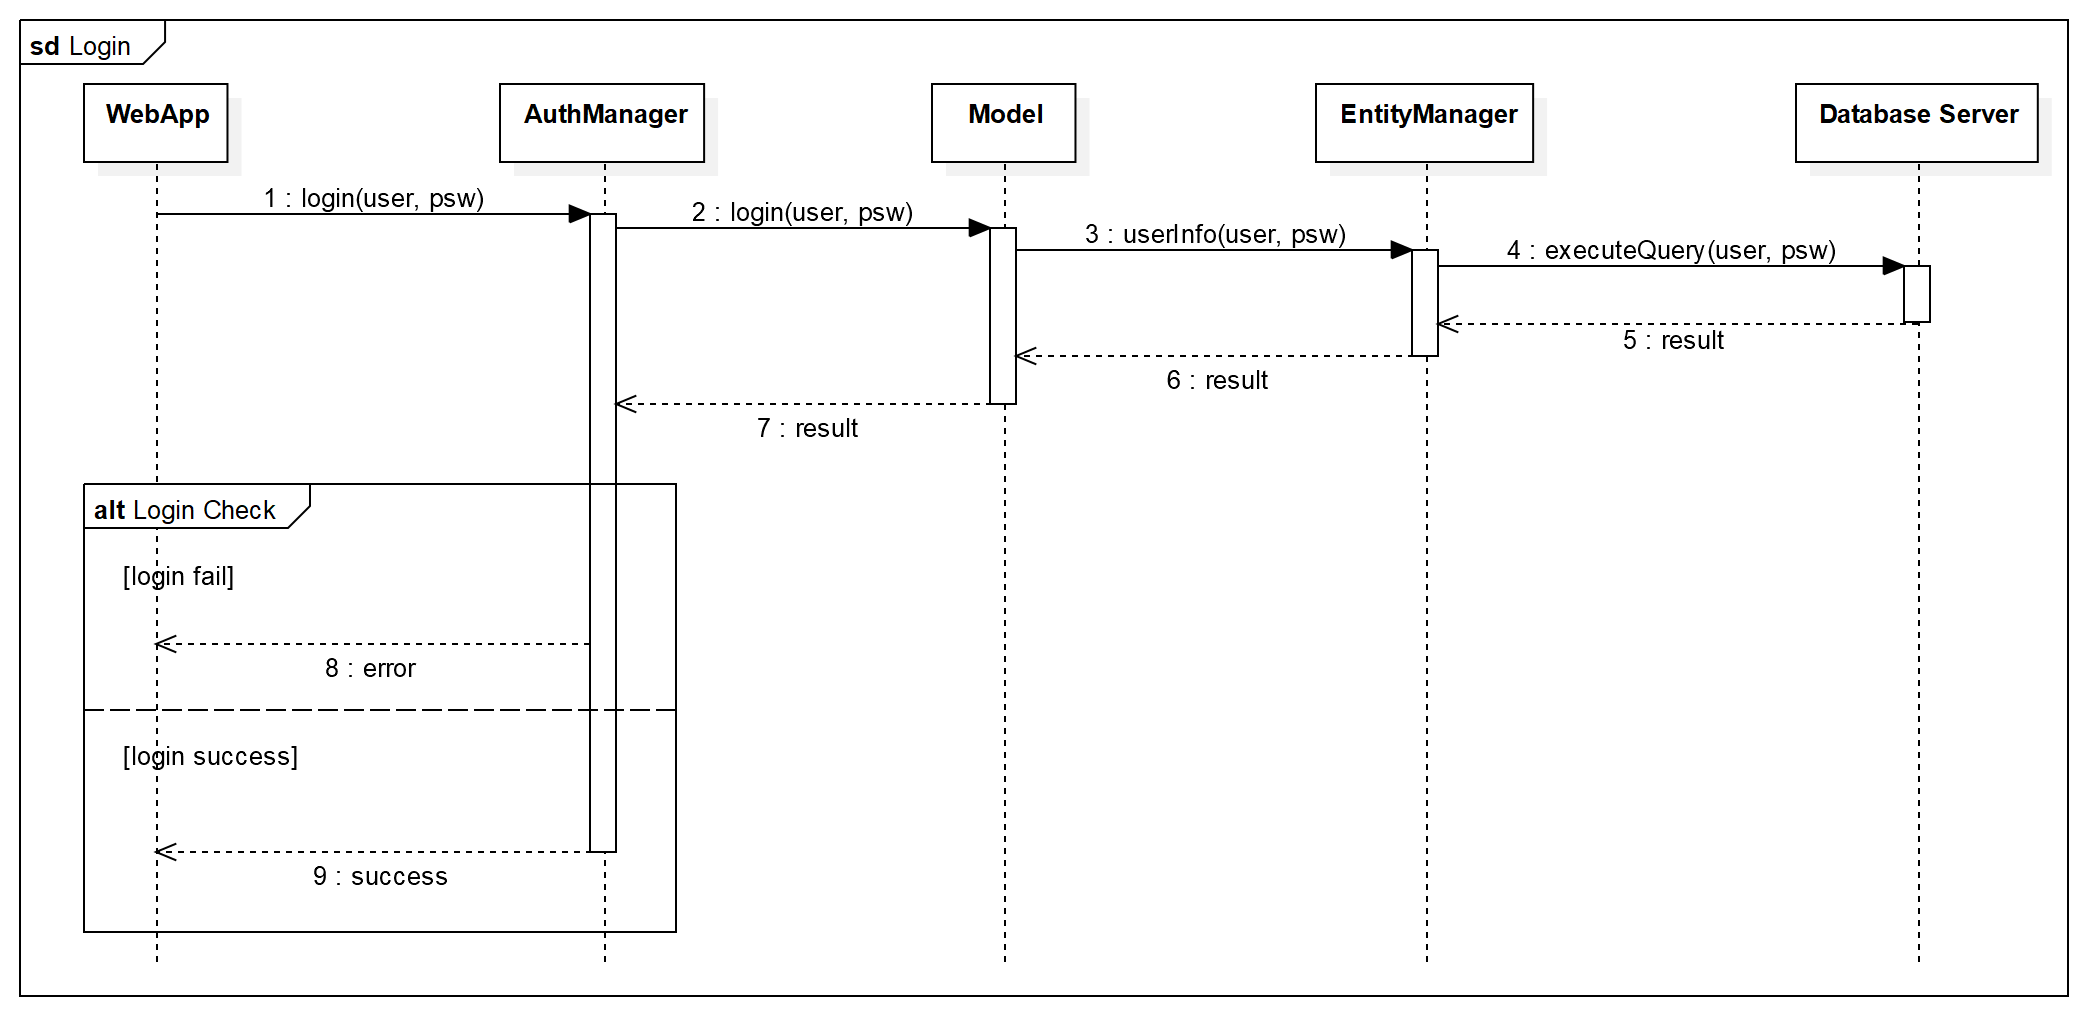
\includegraphics[width=0.75\linewidth]{login_seq}
	\caption{Web App login.}
	\label{fig:login_seq}
\end{figure}

\subsection{Check store status}
After logging in, the store managers can see the store status, for instance the visits booked. The following sequence diagram represents this process. 
\begin{figure}[H]
	\centering
	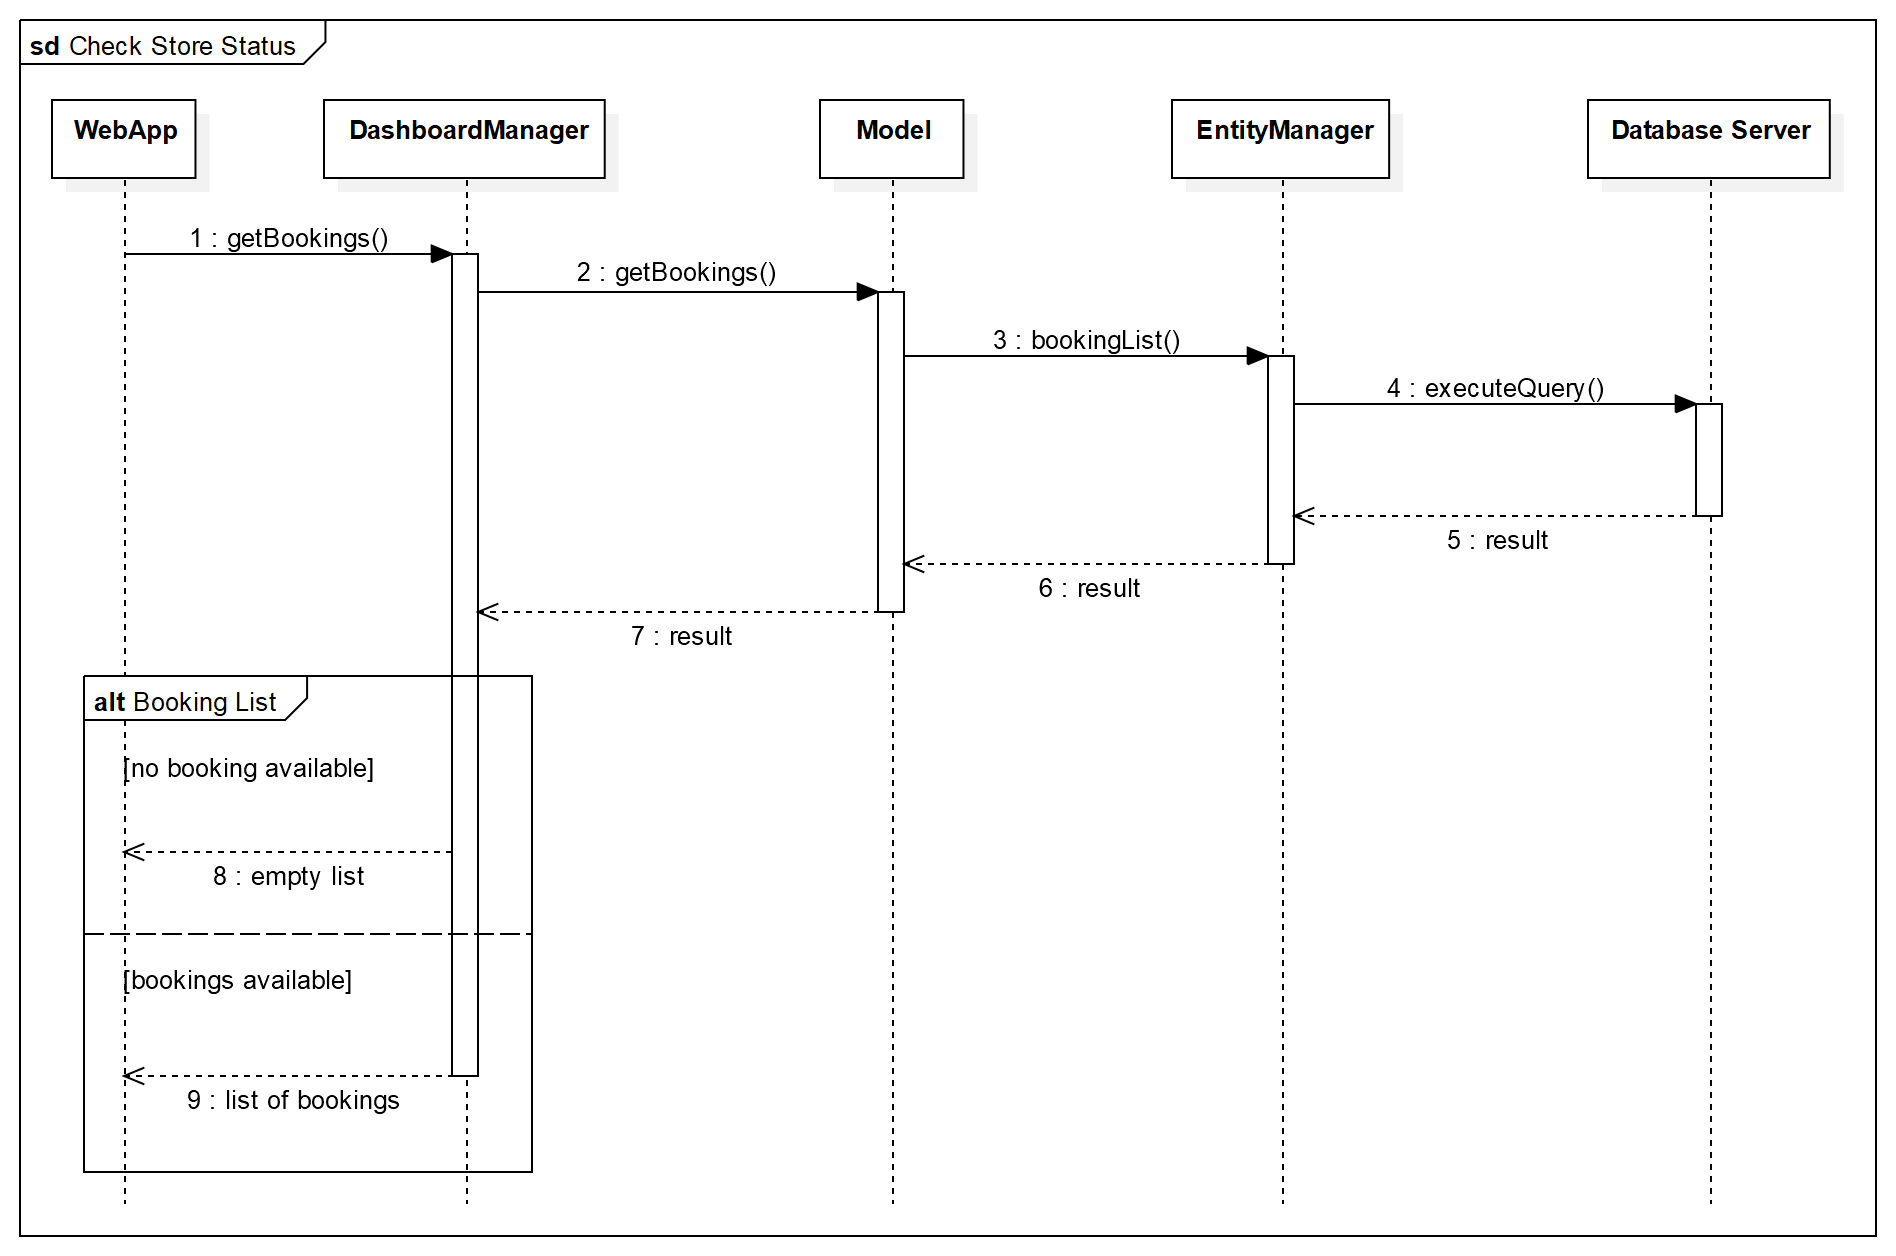
\includegraphics[width=0.75\linewidth]{check_status_seq}
	\caption{Check store status.}
	\label{fig:check_status_seq}
\end{figure}

\subsection{Store App login}
As the Customer App, Store App also has a token to operate. This time there is a login process before the generation of the token.
\begin{figure}[H]
	\centering
	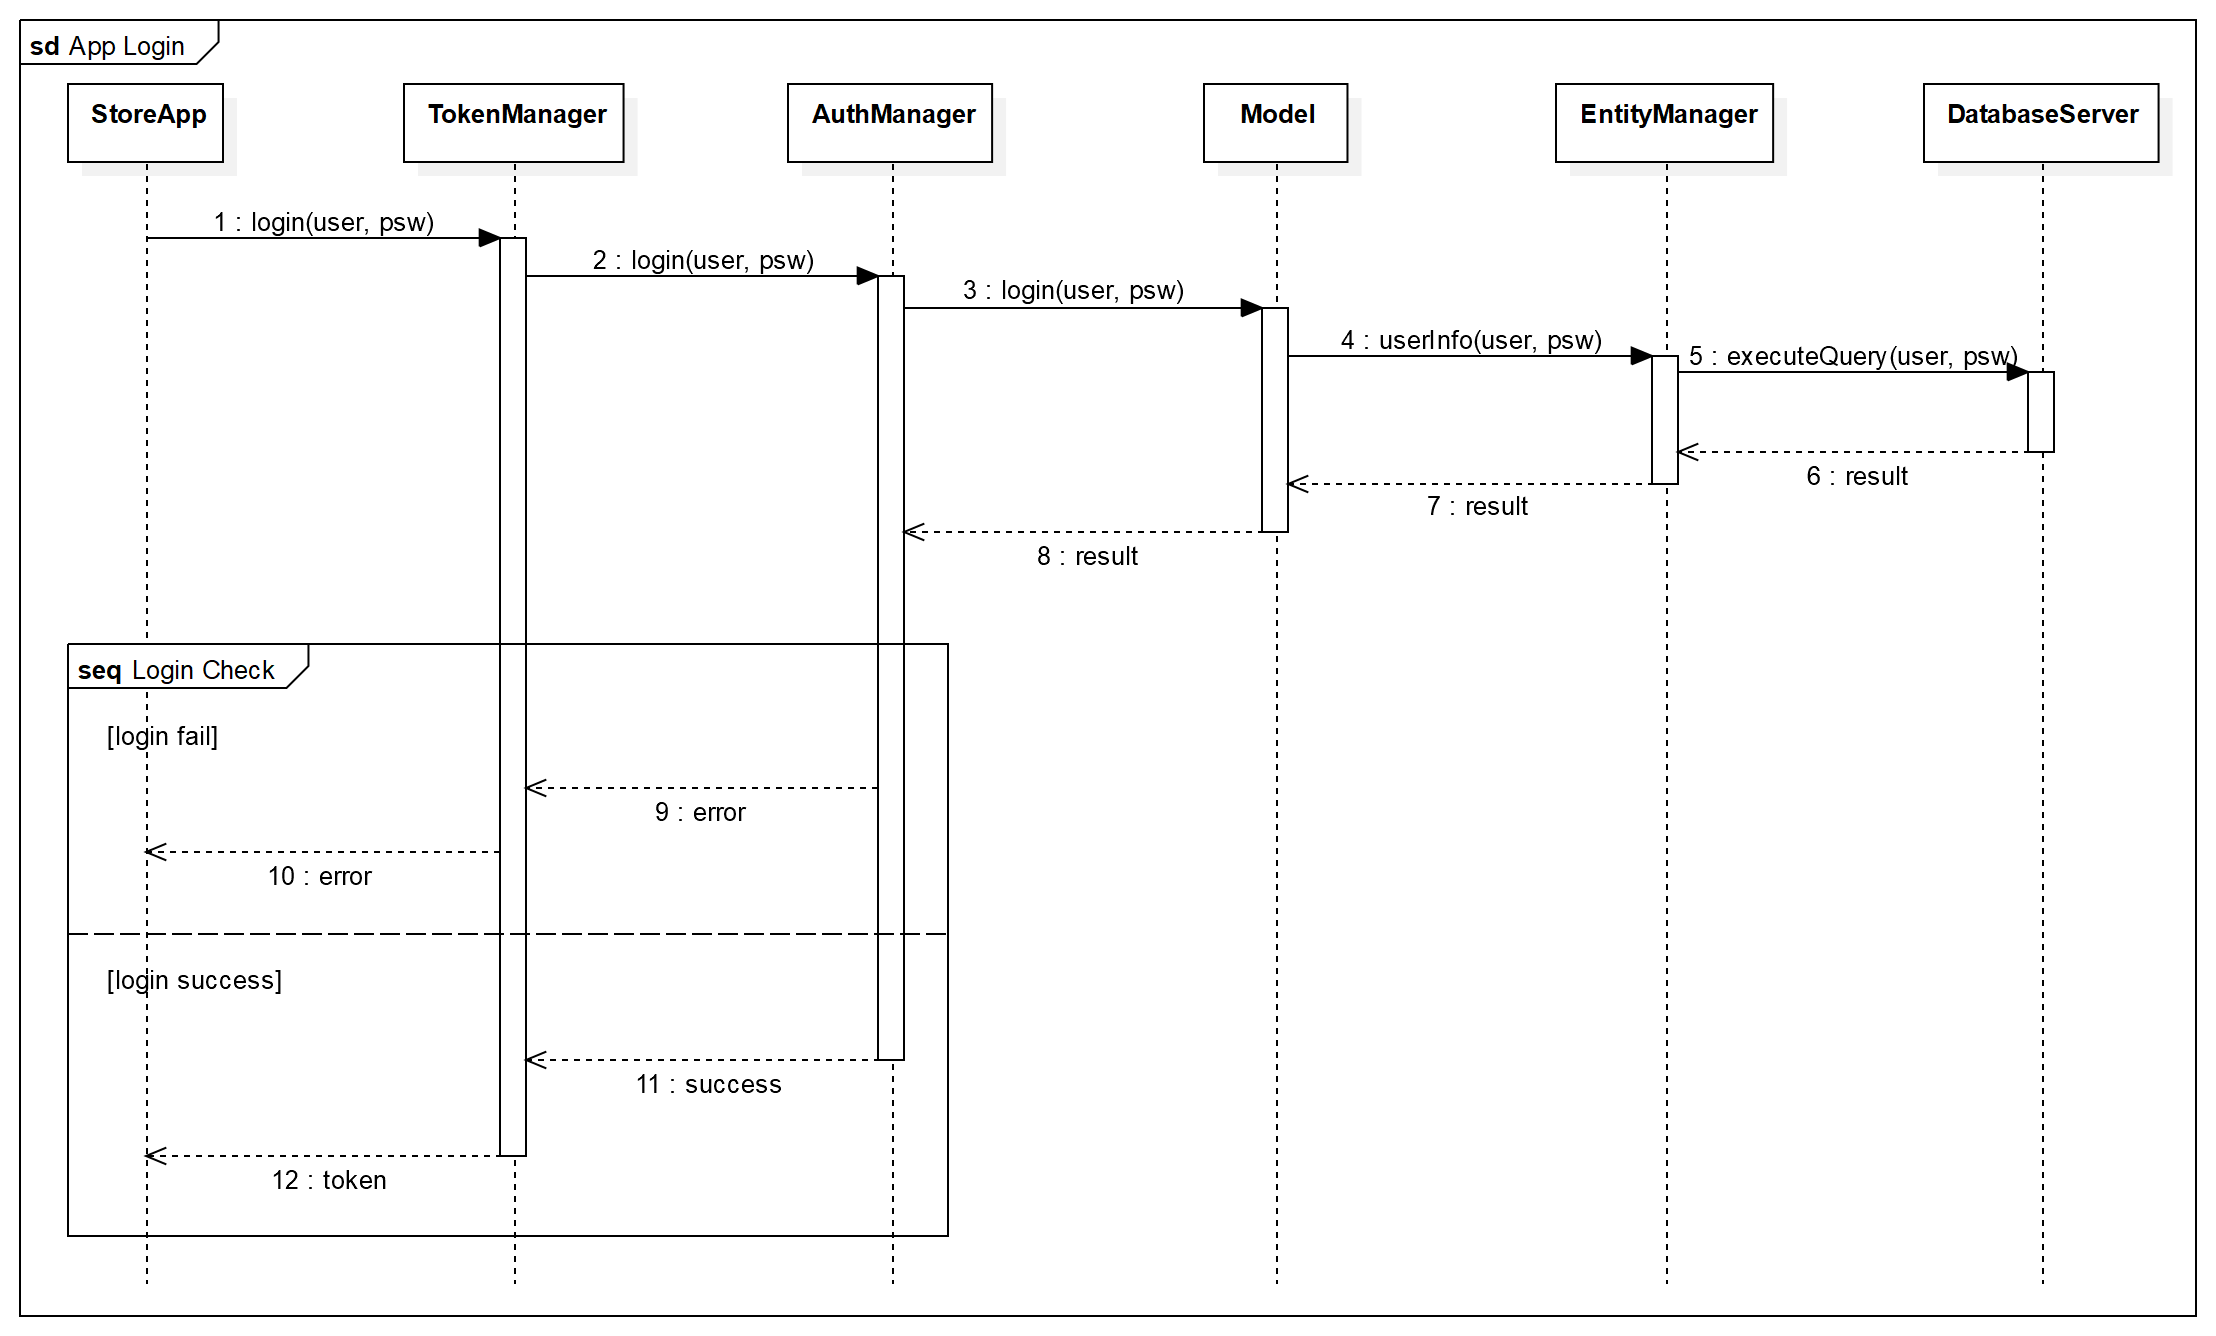
\includegraphics[width=0.75\linewidth]{app_login_seq}
	\caption{Store app login.}
	\label{fig:app_login_seq}
\end{figure}

\subsection{QR Code scan}
The scan of the QR is the most important part of the Store App. After the token validation, the QR code is validated as the sequence diagram shows. If the pass is valid, his status is updated.
\begin{figure}[H]
	\centering
	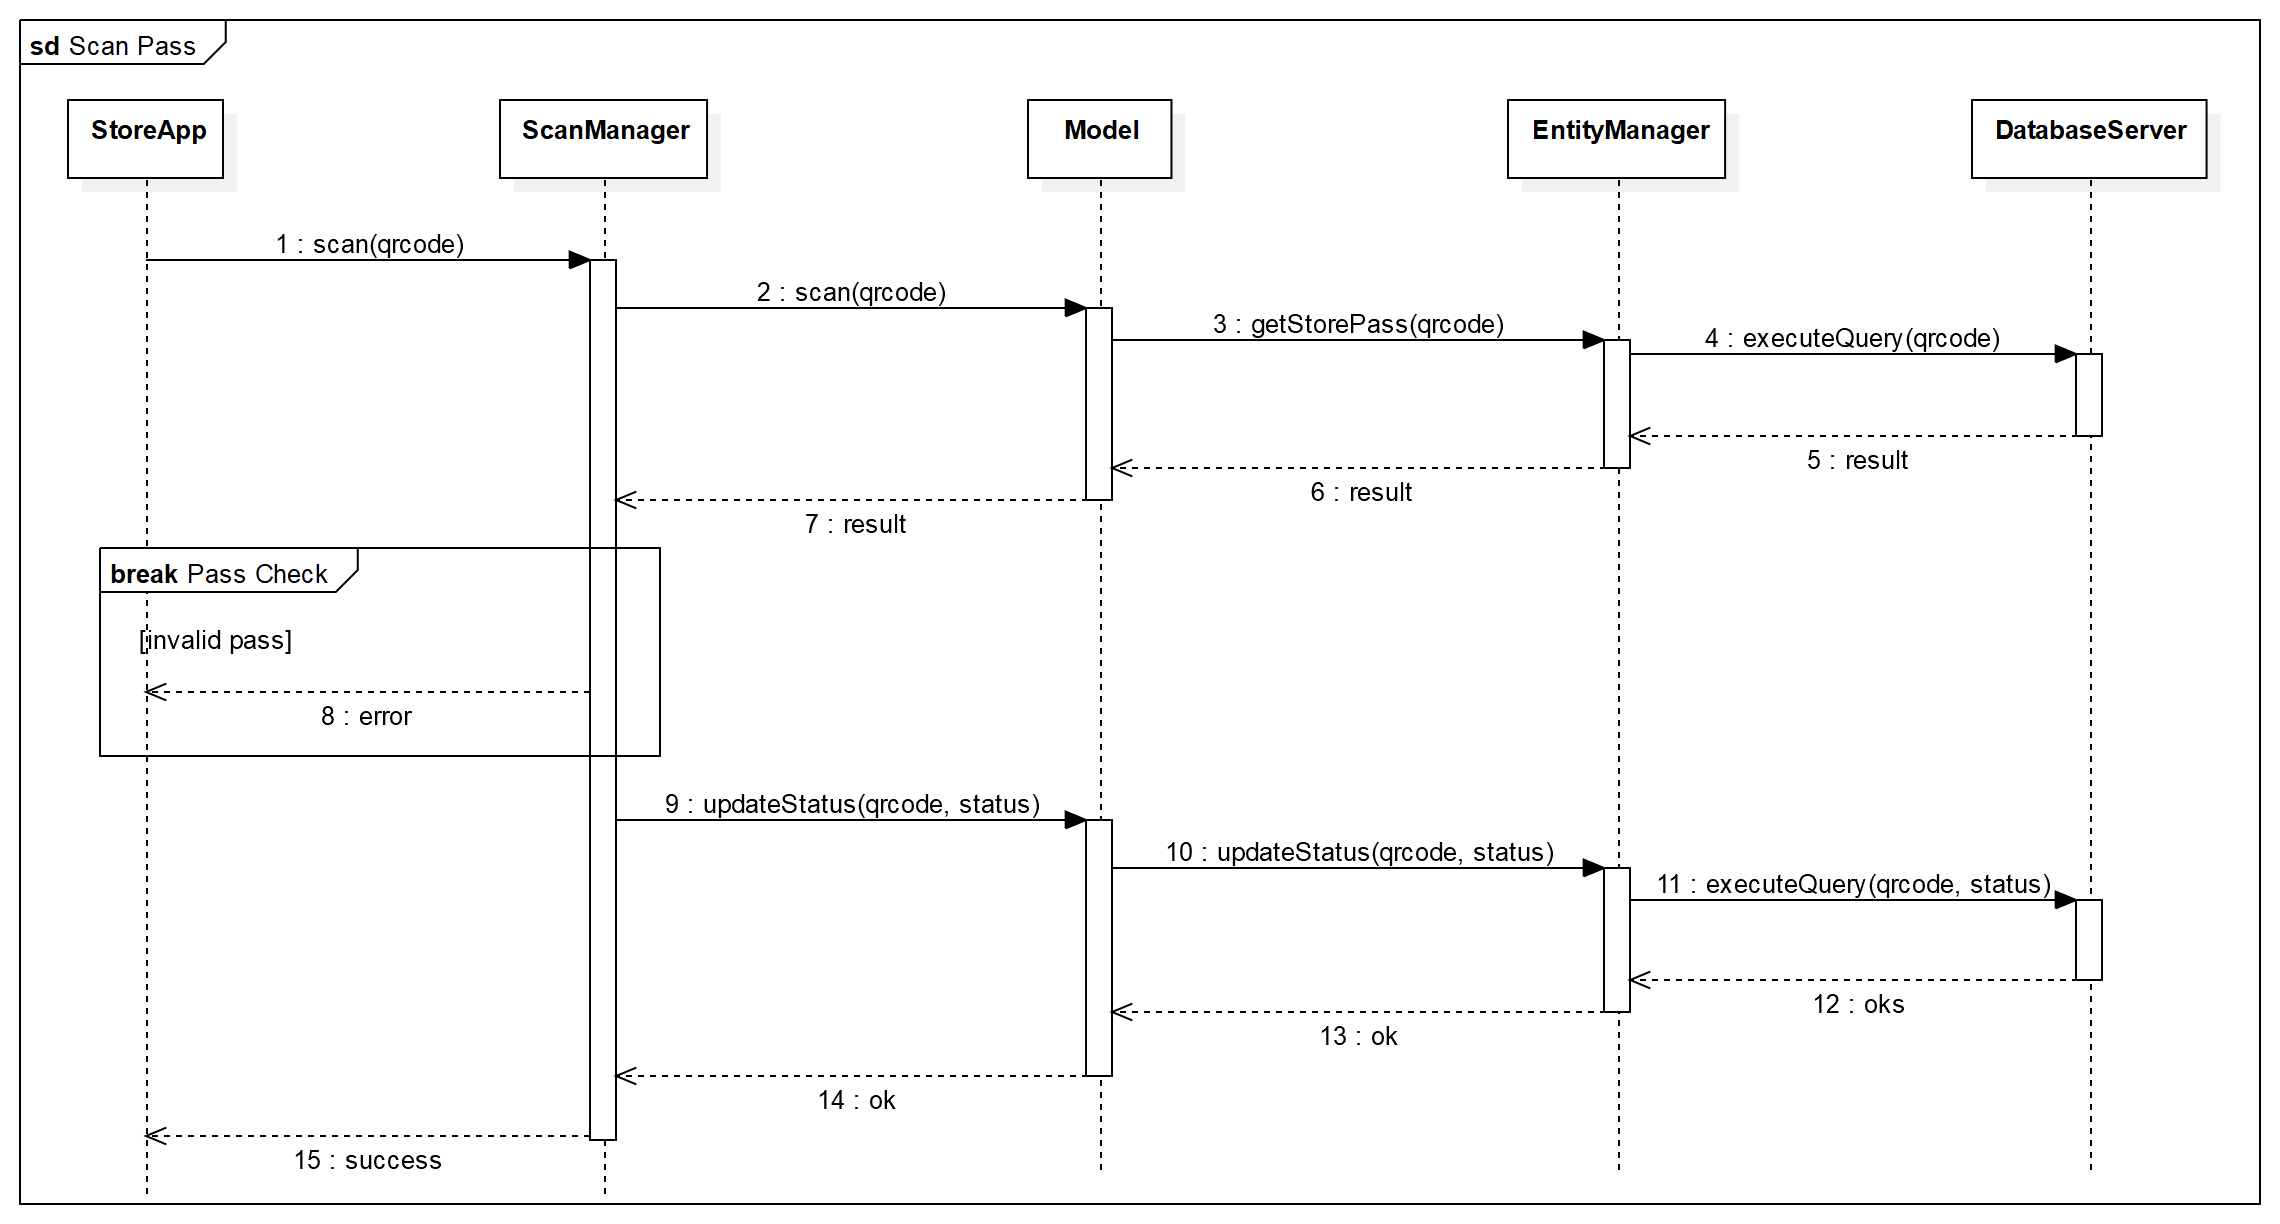
\includegraphics[width=0.85\linewidth]{scan_pass_seq}
	\caption{Store app scan process.}
	\label{fig:scan_pass_seq}
\end{figure}

\subsection{Store registration}
The store registration is performed by a CLup admin via the Web App after his login. Prompted informations are checked from the system and then, if the store doesn't already exist, the store is saved into the database. After that, the credentials for the store managers and store employees are generated and sent to the store PEC address.
\begin{figure}[H]
	\centering
	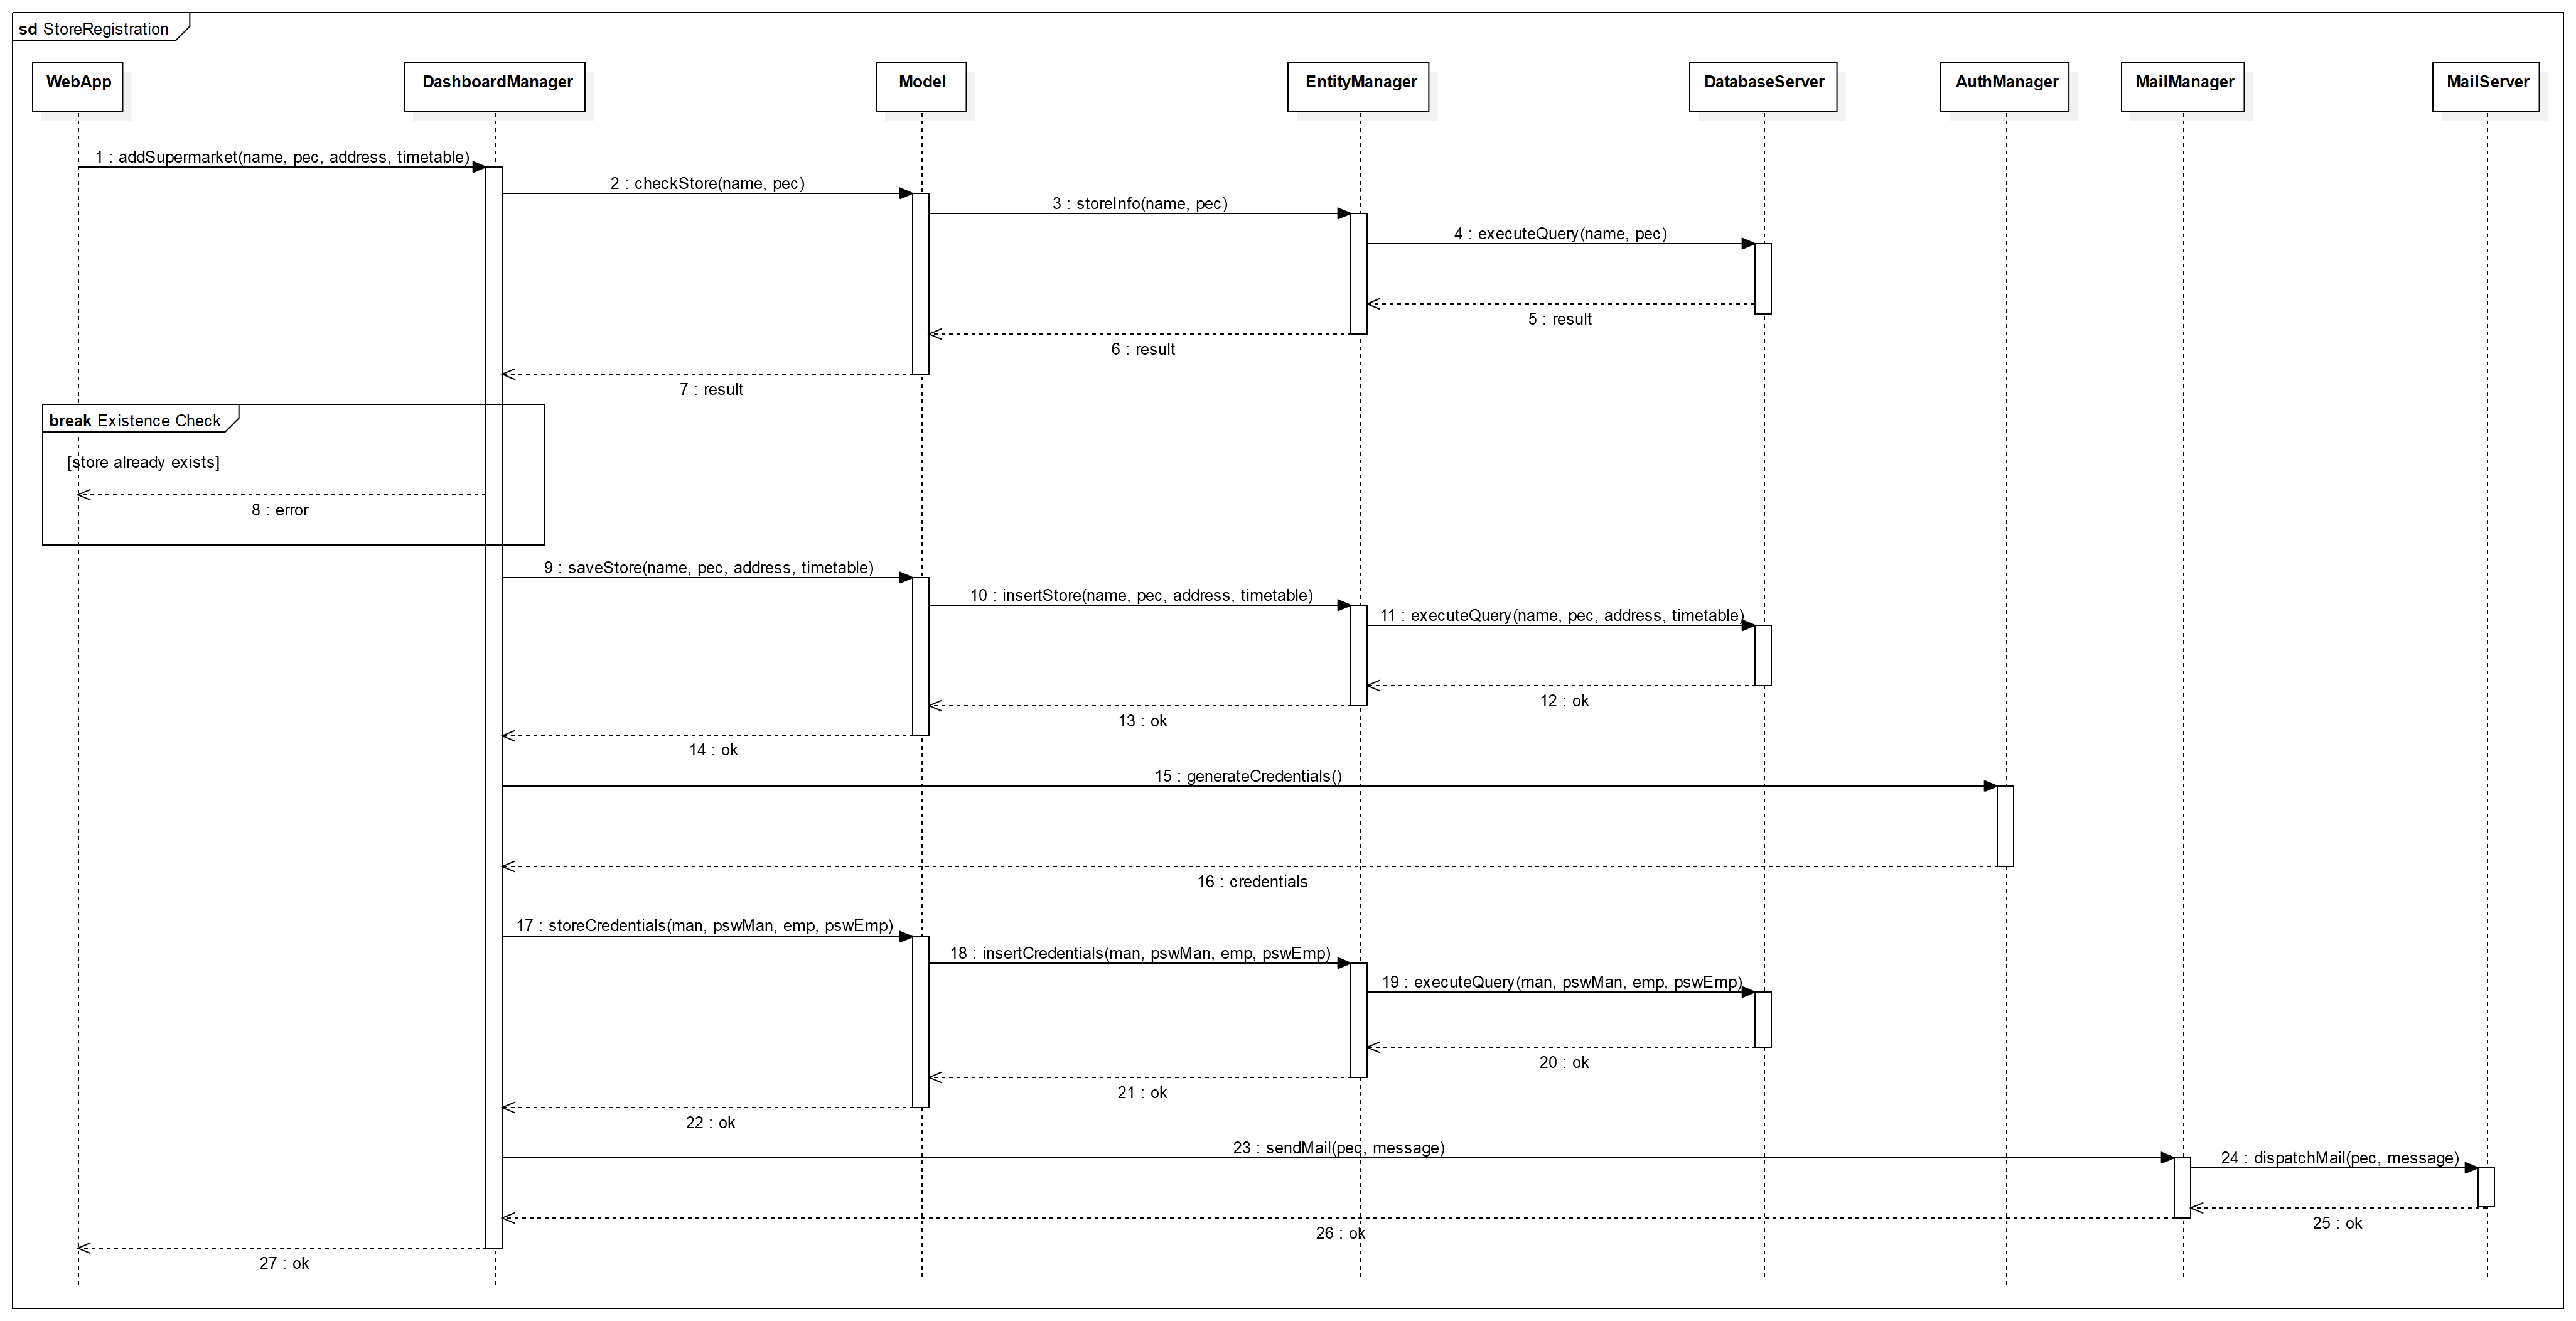
\includegraphics[width=0.85\linewidth]{store_registration_seq}
	\caption{Store registration.}
	\label{fig:store_registration_seq}
\end{figure}

\section{Component interfaces}

\section{Selected architectural styles and patterns}

\section{Other design decisions}
